\documentclass{article}\usepackage[]{graphicx}\usepackage[]{color}
% maxwidth is the original width if it is less than linewidth
% otherwise use linewidth (to make sure the graphics do not exceed the margin)
\makeatletter
\def\maxwidth{ %
  \ifdim\Gin@nat@width>\linewidth
    \linewidth
  \else
    \Gin@nat@width
  \fi
}
\makeatother

\definecolor{fgcolor}{rgb}{0.345, 0.345, 0.345}
\newcommand{\hlnum}[1]{\textcolor[rgb]{0.686,0.059,0.569}{#1}}%
\newcommand{\hlstr}[1]{\textcolor[rgb]{0.192,0.494,0.8}{#1}}%
\newcommand{\hlcom}[1]{\textcolor[rgb]{0.678,0.584,0.686}{\textit{#1}}}%
\newcommand{\hlopt}[1]{\textcolor[rgb]{0,0,0}{#1}}%
\newcommand{\hlstd}[1]{\textcolor[rgb]{0.345,0.345,0.345}{#1}}%
\newcommand{\hlkwa}[1]{\textcolor[rgb]{0.161,0.373,0.58}{\textbf{#1}}}%
\newcommand{\hlkwb}[1]{\textcolor[rgb]{0.69,0.353,0.396}{#1}}%
\newcommand{\hlkwc}[1]{\textcolor[rgb]{0.333,0.667,0.333}{#1}}%
\newcommand{\hlkwd}[1]{\textcolor[rgb]{0.737,0.353,0.396}{\textbf{#1}}}%
\let\hlipl\hlkwb

\usepackage{framed}
\makeatletter
\newenvironment{kframe}{%
 \def\at@end@of@kframe{}%
 \ifinner\ifhmode%
  \def\at@end@of@kframe{\end{minipage}}%
  \begin{minipage}{\columnwidth}%
 \fi\fi%
 \def\FrameCommand##1{\hskip\@totalleftmargin \hskip-\fboxsep
 \colorbox{shadecolor}{##1}\hskip-\fboxsep
     % There is no \\@totalrightmargin, so:
     \hskip-\linewidth \hskip-\@totalleftmargin \hskip\columnwidth}%
 \MakeFramed {\advance\hsize-\width
   \@totalleftmargin\z@ \linewidth\hsize
   \@setminipage}}%
 {\par\unskip\endMakeFramed%
 \at@end@of@kframe}
\makeatother

\definecolor{shadecolor}{rgb}{.97, .97, .97}
\definecolor{messagecolor}{rgb}{0, 0, 0}
\definecolor{warningcolor}{rgb}{1, 0, 1}
\definecolor{errorcolor}{rgb}{1, 0, 0}
\newenvironment{knitrout}{}{} % an empty environment to be redefined in TeX

\usepackage{alltt}
\usepackage[top=1in,bottom=1in,left=1in,right=1in]{geometry}

\usepackage{setspace}

\usepackage{hyperref}
\hypersetup{colorlinks=true, urlcolor=blue, breaklinks=true}

\newcommand{\link}[1]{\footnote{\color{blue}\href{#1}{#1}}}
\newcommand{\myhref}[1]{\href{#1}{#1}}

\usepackage{amsmath}
\usepackage{amssymb}
\usepackage{mathtools}
\usepackage{linguex}
\usepackage{natbib}

%\usepackage{Sweave}





% The package for linguistics examples

\title{Plot and examine chains: 7 regions (no wrap-up; no matrix verb)}
\author{JD}
\IfFileExists{upquote.sty}{\usepackage{upquote}}{}
\begin{document}

\maketitle


\section{Model without emsp}

\begin{knitrout}
\definecolor{shadecolor}{rgb}{0.969, 0.969, 0.969}\color{fgcolor}\begin{kframe}
\begin{alltt}
\hlkwd{library}\hlstd{(dplyr)}
\hlkwd{library}\hlstd{(gdata)}
\hlkwd{library}\hlstd{(ggplot2)}
\hlkwd{library}\hlstd{(ggalt)}

\hlstd{cbPalette} \hlkwb{<-} \hlkwd{c}\hlstd{(}\hlstr{"#E69F00"}\hlstd{,} \hlstr{"#0072B2"}\hlstd{,} \hlstr{"#D55E00"}\hlstd{,} \hlstr{"#CC79A7"}\hlstd{)}

\hlstd{gp} \hlkwb{<-} \hlkwd{read.csv}\hlstd{(}\hlstr{"activations_sentences_gardenpath.csv"}\hlstd{)}

\hlkwd{str}\hlstd{(gp)}
\end{alltt}
\begin{verbatim}
## 'data.frame':	94 obs. of  9 variables:
##  $ activation      : num  2.1 3.18 4.88 6.32 6.38 ...
##  $ position        : int  1 2 3 4 5 6 7 8 1 2 ...
##  $ word            : Factor w/ 36 levels ",",".","a","are",..: 30 19 25 24 30 6 14 2 30 19 ...
##  $ sent_nr         : int  1 1 1 1 1 1 1 1 2 2 ...
##  $ retrieve_wh     : Factor w/ 1 level "None": 1 1 1 1 1 1 1 1 1 1 ...
##  $ reanalysis      : Factor w/ 2 levels "no","yes": 1 1 2 1 1 2 2 1 1 1 ...
##  $ agreeing_actions: num  2 2.5 2.67 3 3 ...
##  $ matching_fs     : num  6.5 6.25 8.83 9 9 ...
##  $ fan_size        : num  1440529 1545912 1426086 1550605 1519423 ...
\end{verbatim}
\begin{alltt}
\hlstd{case1} \hlkwb{<-} \hlkwd{subset}\hlstd{(gp, sent_nr} \hlopt{==} \hlnum{1} \hlopt{|} \hlstd{sent_nr} \hlopt{==} \hlnum{2}\hlstd{)}

\hlkwd{str}\hlstd{(case1)}
\end{alltt}
\begin{verbatim}
## 'data.frame':	18 obs. of  9 variables:
##  $ activation      : num  2.1 3.18 4.88 6.32 6.38 ...
##  $ position        : int  1 2 3 4 5 6 7 8 1 2 ...
##  $ word            : Factor w/ 36 levels ",",".","a","are",..: 30 19 25 24 30 6 14 2 30 19 ...
##  $ sent_nr         : int  1 1 1 1 1 1 1 1 2 2 ...
##  $ retrieve_wh     : Factor w/ 1 level "None": 1 1 1 1 1 1 1 1 1 1 ...
##  $ reanalysis      : Factor w/ 2 levels "no","yes": 1 1 2 1 1 2 2 1 1 1 ...
##  $ agreeing_actions: num  2 2.5 2.67 3 3 ...
##  $ matching_fs     : num  6.5 6.25 8.83 9 9 ...
##  $ fan_size        : num  1440529 1545912 1426086 1550605 1519423 ...
\end{verbatim}
\begin{alltt}
\hlstd{case1}\hlopt{$}\hlstd{word} \hlkwb{<-} \hlkwd{as.character}\hlstd{(case1}\hlopt{$}\hlstd{word)}

\hlstd{case1}\hlopt{$}\hlstd{word[}\hlkwd{which}\hlstd{(case1}\hlopt{$}\hlstd{position} \hlopt{==} \hlnum{5} \hlopt{&} \hlstd{case1}\hlopt{$}\hlstd{sent_nr} \hlopt{==} \hlnum{1}\hlstd{)]} \hlkwb{<-} \hlstr{"the "}
\hlstd{case1}\hlopt{$}\hlstd{word[}\hlkwd{which}\hlstd{(case1}\hlopt{$}\hlstd{position} \hlopt{==} \hlnum{7} \hlopt{&} \hlstd{case1}\hlopt{$}\hlstd{sent_nr} \hlopt{==} \hlnum{2}\hlstd{)]} \hlkwb{<-} \hlstr{"the "}
\hlstd{case1}\hlopt{$}\hlstd{word[}\hlkwd{which}\hlstd{(case1}\hlopt{$}\hlstd{word} \hlopt{==} \hlstr{"which"}\hlstd{)]} \hlkwb{<-} \hlstr{"(which)"}
\hlstd{case1}\hlopt{$}\hlstd{word[}\hlkwd{which}\hlstd{(case1}\hlopt{$}\hlstd{word} \hlopt{==} \hlstr{"was"}\hlstd{)]} \hlkwb{<-} \hlstr{"(was)"}

\hlstd{case1}\hlopt{$}\hlstd{word} \hlkwb{<-} \hlkwd{as.factor}\hlstd{(}\hlkwd{as.character}\hlstd{(case1}\hlopt{$}\hlstd{word))}
\hlkwd{levels}\hlstd{(case1}\hlopt{$}\hlstd{word)}
\end{alltt}
\begin{verbatim}
##  [1] "."       "(was)"   "(which)" "barn"    "fell"    "horse"   "past"   
##  [8] "raced"   "the"     "the "
\end{verbatim}
\begin{alltt}
\hlstd{case1}\hlopt{$}\hlstd{garden_path} \hlkwb{<-} \hlstr{"no"}
\hlstd{case1}\hlopt{$}\hlstd{garden_path[}\hlkwd{which}\hlstd{(case1}\hlopt{$}\hlstd{sent} \hlopt{==} \hlnum{1}\hlstd{)]} \hlkwb{<-} \hlstr{"yes"}

\hlcom{# fake missing words with 0 for nice graphs}
\hlstd{case1} \hlkwb{<-} \hlkwd{rbind}\hlstd{(case1,} \hlkwd{data.frame}\hlstd{(}\hlkwc{activation} \hlstd{=} \hlnum{0}\hlstd{,} \hlkwc{position} \hlstd{=} \hlnum{0}\hlstd{,} \hlkwc{word} \hlstd{=} \hlstr{"(which)"}\hlstd{,}
    \hlkwc{sent_nr} \hlstd{=} \hlnum{1}\hlstd{,} \hlkwc{retrieve_wh} \hlstd{=} \hlstr{"None"}\hlstd{,} \hlkwc{reanalysis} \hlstd{=} \hlstr{"no"}\hlstd{,} \hlkwc{agreeing_actions} \hlstd{=} \hlnum{0}\hlstd{,}
    \hlkwc{matching_fs} \hlstd{=} \hlnum{0}\hlstd{,} \hlkwc{fan_size} \hlstd{=} \hlnum{0}\hlstd{,} \hlkwc{garden_path} \hlstd{=} \hlstr{"yes"}\hlstd{))}
\hlstd{case1} \hlkwb{<-} \hlkwd{rbind}\hlstd{(case1,} \hlkwd{data.frame}\hlstd{(}\hlkwc{activation} \hlstd{=} \hlnum{0}\hlstd{,} \hlkwc{position} \hlstd{=} \hlnum{0}\hlstd{,} \hlkwc{word} \hlstd{=} \hlstr{"(was)"}\hlstd{,}
    \hlkwc{sent_nr} \hlstd{=} \hlnum{1}\hlstd{,} \hlkwc{retrieve_wh} \hlstd{=} \hlstr{"None"}\hlstd{,} \hlkwc{reanalysis} \hlstd{=} \hlstr{"no"}\hlstd{,} \hlkwc{agreeing_actions} \hlstd{=} \hlnum{0}\hlstd{,}
    \hlkwc{matching_fs} \hlstd{=} \hlnum{0}\hlstd{,} \hlkwc{fan_size} \hlstd{=} \hlnum{0}\hlstd{,} \hlkwc{garden_path} \hlstd{=} \hlstr{"yes"}\hlstd{))}

\hlcom{# find which word should be circled as causing gp}
\hlstd{case1}\hlopt{$}\hlstd{gp} \hlkwb{<-} \hlnum{NA}
\hlstd{case1}\hlopt{$}\hlstd{gp[}\hlkwd{which}\hlstd{(case1}\hlopt{$}\hlstd{word} \hlopt{==} \hlstr{"fell"}\hlstd{)]} \hlkwb{<-} \hlstr{"yes"}

\hlcom{# case1$word <- drop.levels(case1$word)}

\hlstd{ordered_levels} \hlkwb{<-} \hlkwd{as.numeric}\hlstd{(}\hlkwd{subset}\hlstd{(case1, sent_nr} \hlopt{==} \hlnum{2}\hlstd{)}\hlopt{$}\hlstd{word)}

\hlstd{case1}\hlopt{$}\hlstd{word} \hlkwb{<-} \hlkwd{factor}\hlstd{(case1}\hlopt{$}\hlstd{word,} \hlkwd{levels}\hlstd{(case1}\hlopt{$}\hlstd{word)[ordered_levels])}
\hlkwd{levels}\hlstd{(case1}\hlopt{$}\hlstd{word)}
\end{alltt}
\begin{verbatim}
##  [1] "the"     "horse"   "(which)" "(was)"   "raced"   "past"    "the "   
##  [8] "barn"    "fell"    "."
\end{verbatim}
\begin{alltt}
\hlkwd{str}\hlstd{(case1)}
\end{alltt}
\begin{verbatim}
## 'data.frame':	20 obs. of  11 variables:
##  $ activation      : num  2.1 3.18 4.88 6.32 6.38 ...
##  $ position        : num  1 2 3 4 5 6 7 8 1 2 ...
##  $ word            : Factor w/ 10 levels "the","horse",..: 1 2 5 6 7 8 9 10 1 2 ...
##  $ sent_nr         : num  1 1 1 1 1 1 1 1 2 2 ...
##  $ retrieve_wh     : Factor w/ 1 level "None": 1 1 1 1 1 1 1 1 1 1 ...
##  $ reanalysis      : Factor w/ 2 levels "no","yes": 1 1 2 1 1 2 2 1 1 1 ...
##  $ agreeing_actions: num  2 2.5 2.67 3 3 ...
##  $ matching_fs     : num  6.5 6.25 8.83 9 9 ...
##  $ fan_size        : num  1440529 1545912 1426086 1550605 1519423 ...
##  $ garden_path     : chr  "yes" "yes" "yes" "yes" ...
##  $ gp              : chr  NA NA NA NA ...
\end{verbatim}
\begin{alltt}
\hlstd{g1} \hlkwb{<-} \hlkwd{ggplot}\hlstd{(case1,} \hlkwd{aes}\hlstd{(}\hlkwc{x} \hlstd{= word,} \hlkwc{y} \hlstd{= activation,} \hlkwc{fill} \hlstd{= garden_path,} \hlkwc{group} \hlstd{= garden_path))}
\hlstd{g1} \hlkwb{<-} \hlstd{g1} \hlopt{+} \hlkwd{geom_bar}\hlstd{(}\hlkwc{stat} \hlstd{=} \hlstr{"identity"}\hlstd{,} \hlkwc{position} \hlstd{=} \hlstr{"dodge"}\hlstd{)}
\hlstd{g1} \hlkwb{<-} \hlstd{g1} \hlopt{+} \hlkwd{geom_encircle}\hlstd{(}\hlkwc{data} \hlstd{=} \hlkwd{subset}\hlstd{(case1, gp} \hlopt{==} \hlstr{"yes"}\hlstd{),} \hlkwd{aes}\hlstd{(word, activation),}
    \hlkwc{inherit.aes} \hlstd{=} \hlnum{FALSE}\hlstd{,} \hlkwc{s_shape} \hlstd{=} \hlnum{0}\hlstd{,} \hlkwc{spread} \hlstd{=} \hlnum{0.05}\hlstd{,} \hlkwc{size} \hlstd{=} \hlnum{3}\hlstd{,} \hlkwc{color} \hlstd{=} \hlstr{"#D55E00"}\hlstd{)}
\hlstd{g1} \hlkwb{<-} \hlstd{g1} \hlopt{+} \hlkwd{theme_gray}\hlstd{(}\hlnum{26}\hlstd{)} \hlopt{+} \hlkwd{scale_fill_manual}\hlstd{(}\hlkwc{values} \hlstd{= cbPalette)}
\end{alltt}
\end{kframe}
\end{knitrout}

\begin{knitrout}
\definecolor{shadecolor}{rgb}{0.969, 0.969, 0.969}\color{fgcolor}
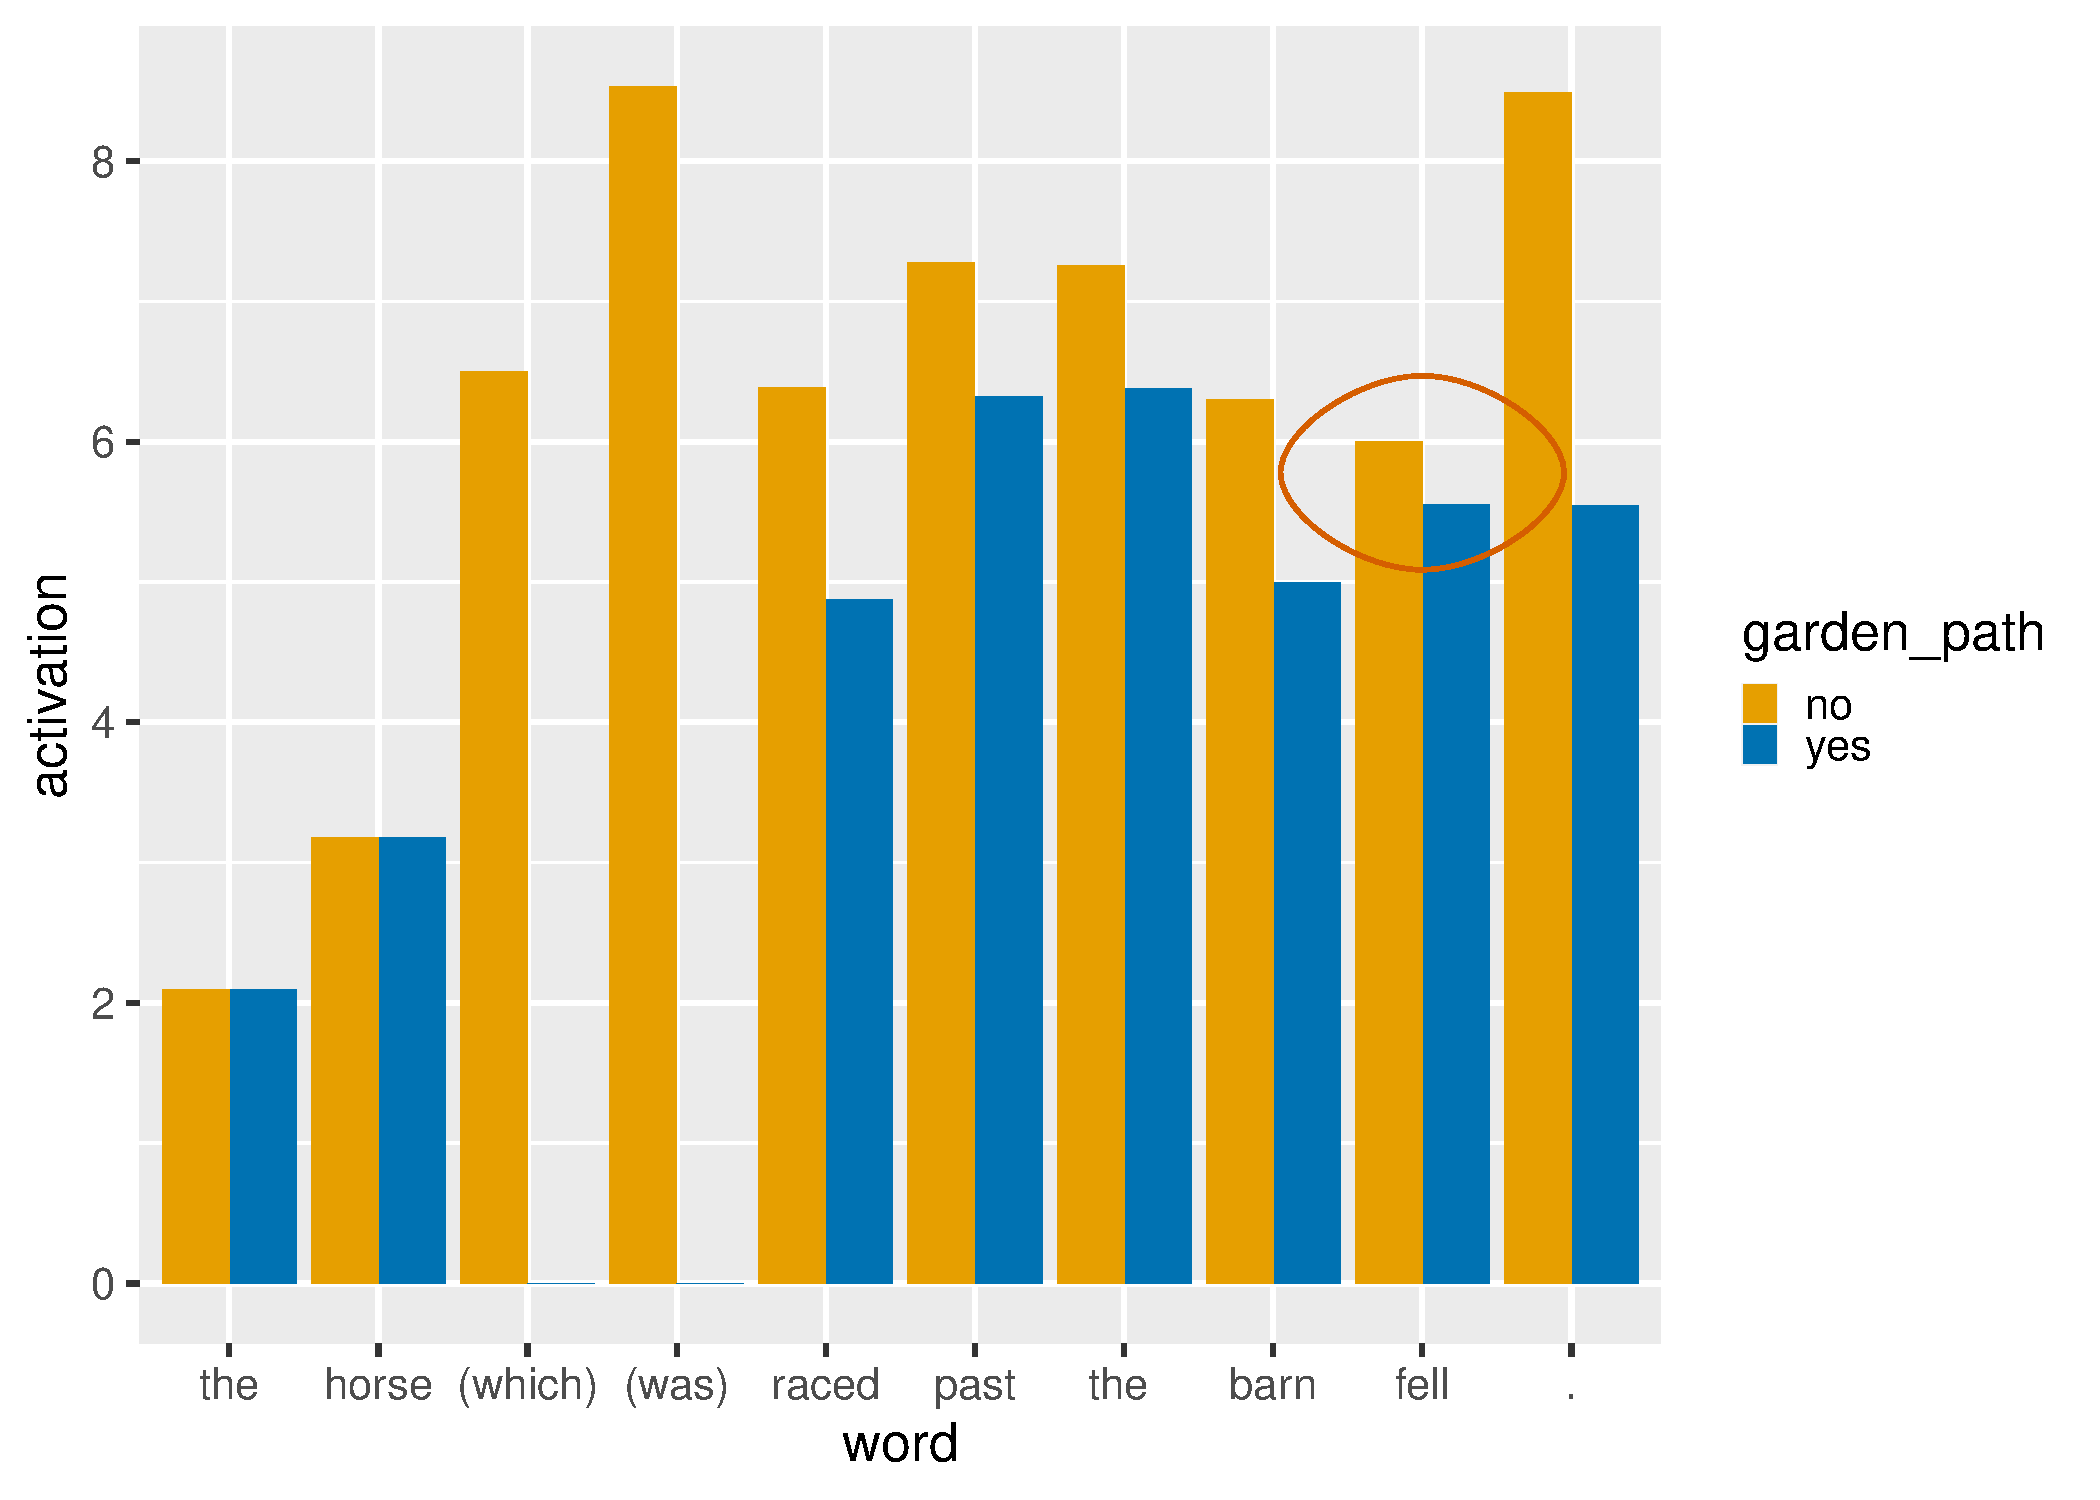
\includegraphics[width=\maxwidth]{figures/unnamed-chunk-4-1} 

\end{knitrout}

\begin{knitrout}
\definecolor{shadecolor}{rgb}{0.969, 0.969, 0.969}\color{fgcolor}\begin{kframe}
\begin{alltt}
\hlstd{case2} \hlkwb{<-} \hlkwd{subset}\hlstd{(gp, sent_nr} \hlopt{==} \hlnum{3} \hlopt{|} \hlstd{sent_nr} \hlopt{==} \hlnum{4}\hlstd{)}

\hlkwd{str}\hlstd{(case2)}
\end{alltt}
\begin{verbatim}
## 'data.frame':	21 obs. of  9 variables:
##  $ activation      : num  2.31 3.74 7.55 6.67 7.32 ...
##  $ position        : int  1 2 3 4 5 6 7 8 9 10 ...
##  $ word            : Factor w/ 36 levels ",",".","a","are",..: 34 27 21 30 28 14 23 30 15 2 ...
##  $ sent_nr         : int  3 3 3 3 3 3 3 3 3 3 ...
##  $ retrieve_wh     : Factor w/ 1 level "None": 1 1 1 1 1 1 1 1 1 1 ...
##  $ reanalysis      : Factor w/ 2 levels "no","yes": 1 1 1 1 1 2 1 1 2 1 ...
##  $ agreeing_actions: num  2 2.5 3 2 3 ...
##  $ matching_fs     : num  7 6.67 9 17.5 9.33 ...
##  $ fan_size        : num  1322830 1405593 1405410 764278 1430089 ...
\end{verbatim}
\begin{alltt}
\hlstd{case2}\hlopt{$}\hlstd{word} \hlkwb{<-} \hlkwd{as.character}\hlstd{(case2}\hlopt{$}\hlstd{word)}

\hlstd{case2}\hlopt{$}\hlstd{word[}\hlkwd{which}\hlstd{(case2}\hlopt{$}\hlstd{position} \hlopt{==} \hlnum{8} \hlopt{&} \hlstd{case2}\hlopt{$}\hlstd{sent_nr} \hlopt{==} \hlnum{3}\hlstd{)]} \hlkwb{<-} \hlstr{"the "}
\hlstd{case2}\hlopt{$}\hlstd{word[}\hlkwd{which}\hlstd{(case2}\hlopt{$}\hlstd{position} \hlopt{==} \hlnum{9} \hlopt{&} \hlstd{case2}\hlopt{$}\hlstd{sent_nr} \hlopt{==} \hlnum{4}\hlstd{)]} \hlkwb{<-} \hlstr{"the "}
\hlstd{case2}\hlopt{$}\hlstd{word[}\hlkwd{which}\hlstd{(case2}\hlopt{$}\hlstd{word} \hlopt{==} \hlstr{","}\hlstd{)]} \hlkwb{<-} \hlstr{"(,)"}

\hlstd{case2}\hlopt{$}\hlstd{word} \hlkwb{<-} \hlkwd{as.factor}\hlstd{(}\hlkwd{as.character}\hlstd{(case2}\hlopt{$}\hlstd{word))}
\hlkwd{levels}\hlstd{(case2}\hlopt{$}\hlstd{word)}
\end{alltt}
\begin{verbatim}
##  [1] "."      "(,)"    "fell"   "floor"  "mended" "on"     "she"   
##  [8] "sock"   "the"    "the "   "while"
\end{verbatim}
\begin{alltt}
\hlstd{case2}\hlopt{$}\hlstd{garden_path} \hlkwb{<-} \hlstr{"no"}
\hlstd{case2}\hlopt{$}\hlstd{garden_path[}\hlkwd{which}\hlstd{(case2}\hlopt{$}\hlstd{sent} \hlopt{==} \hlnum{3}\hlstd{)]} \hlkwb{<-} \hlstr{"yes"}

\hlstd{case2} \hlkwb{<-} \hlkwd{rbind}\hlstd{(case2,} \hlkwd{data.frame}\hlstd{(}\hlkwc{activation} \hlstd{=} \hlnum{0}\hlstd{,} \hlkwc{position} \hlstd{=} \hlnum{0}\hlstd{,} \hlkwc{word} \hlstd{=} \hlstr{"(,)"}\hlstd{,}
    \hlkwc{sent_nr} \hlstd{=} \hlnum{3}\hlstd{,} \hlkwc{retrieve_wh} \hlstd{=} \hlstr{"None"}\hlstd{,} \hlkwc{reanalysis} \hlstd{=} \hlstr{"no"}\hlstd{,} \hlkwc{agreeing_actions} \hlstd{=} \hlnum{0}\hlstd{,}
    \hlkwc{matching_fs} \hlstd{=} \hlnum{0}\hlstd{,} \hlkwc{fan_size} \hlstd{=} \hlnum{0}\hlstd{,} \hlkwc{garden_path} \hlstd{=} \hlstr{"yes"}\hlstd{))}

\hlstd{case2}\hlopt{$}\hlstd{gp} \hlkwb{<-} \hlnum{NA}
\hlstd{case2}\hlopt{$}\hlstd{gp[}\hlkwd{which}\hlstd{(case2}\hlopt{$}\hlstd{word} \hlopt{==} \hlstr{"fell"}\hlstd{)]} \hlkwb{<-} \hlstr{"yes"}

\hlstd{ordered_levels} \hlkwb{<-} \hlkwd{as.numeric}\hlstd{(}\hlkwd{subset}\hlstd{(case2, sent_nr} \hlopt{==} \hlnum{4}\hlstd{)}\hlopt{$}\hlstd{word)}

\hlstd{case2}\hlopt{$}\hlstd{word} \hlkwb{<-} \hlkwd{factor}\hlstd{(case2}\hlopt{$}\hlstd{word,} \hlkwd{levels}\hlstd{(case2}\hlopt{$}\hlstd{word)[ordered_levels])}
\hlkwd{levels}\hlstd{(case2}\hlopt{$}\hlstd{word)}
\end{alltt}
\begin{verbatim}
##  [1] "while"  "she"    "mended" "(,)"    "the"    "sock"   "fell"  
##  [8] "on"     "the "   "floor"  "."
\end{verbatim}
\begin{alltt}
\hlkwd{str}\hlstd{(case2)}
\end{alltt}
\begin{verbatim}
## 'data.frame':	22 obs. of  11 variables:
##  $ activation      : num  2.31 3.74 7.55 6.67 7.32 ...
##  $ position        : num  1 2 3 4 5 6 7 8 9 10 ...
##  $ word            : Factor w/ 11 levels "while","she",..: 1 2 3 5 6 7 8 9 10 11 ...
##  $ sent_nr         : num  3 3 3 3 3 3 3 3 3 3 ...
##  $ retrieve_wh     : Factor w/ 1 level "None": 1 1 1 1 1 1 1 1 1 1 ...
##  $ reanalysis      : Factor w/ 2 levels "no","yes": 1 1 1 1 1 2 1 1 2 1 ...
##  $ agreeing_actions: num  2 2.5 3 2 3 ...
##  $ matching_fs     : num  7 6.67 9 17.5 9.33 ...
##  $ fan_size        : num  1322830 1405593 1405410 764278 1430089 ...
##  $ garden_path     : chr  "yes" "yes" "yes" "yes" ...
##  $ gp              : chr  NA NA NA NA ...
\end{verbatim}
\begin{alltt}
\hlstd{g1} \hlkwb{<-} \hlkwd{ggplot}\hlstd{(case2,} \hlkwd{aes}\hlstd{(}\hlkwc{x} \hlstd{= word,} \hlkwc{y} \hlstd{= activation,} \hlkwc{fill} \hlstd{= garden_path,} \hlkwc{group} \hlstd{= garden_path))}
\hlstd{g1} \hlkwb{<-} \hlstd{g1} \hlopt{+} \hlkwd{geom_bar}\hlstd{(}\hlkwc{stat} \hlstd{=} \hlstr{"identity"}\hlstd{,} \hlkwc{position} \hlstd{=} \hlstr{"dodge"}\hlstd{)}
\hlstd{g1} \hlkwb{<-} \hlstd{g1} \hlopt{+} \hlkwd{geom_encircle}\hlstd{(}\hlkwc{data} \hlstd{=} \hlkwd{subset}\hlstd{(case2, gp} \hlopt{==} \hlstr{"yes"}\hlstd{),} \hlkwd{aes}\hlstd{(word, activation),}
    \hlkwc{inherit.aes} \hlstd{=} \hlnum{FALSE}\hlstd{,} \hlkwc{s_shape} \hlstd{=} \hlnum{0}\hlstd{,} \hlkwc{spread} \hlstd{=} \hlnum{0.02}\hlstd{,} \hlkwc{size} \hlstd{=} \hlnum{3}\hlstd{,} \hlkwc{color} \hlstd{=} \hlstr{"#D55E00"}\hlstd{)}
\hlstd{g1} \hlkwb{<-} \hlstd{g1} \hlopt{+} \hlkwd{theme_gray}\hlstd{(}\hlnum{26}\hlstd{)} \hlopt{+} \hlkwd{scale_fill_manual}\hlstd{(}\hlkwc{values} \hlstd{= cbPalette)}
\end{alltt}
\end{kframe}
\end{knitrout}

\begin{knitrout}
\definecolor{shadecolor}{rgb}{0.969, 0.969, 0.969}\color{fgcolor}
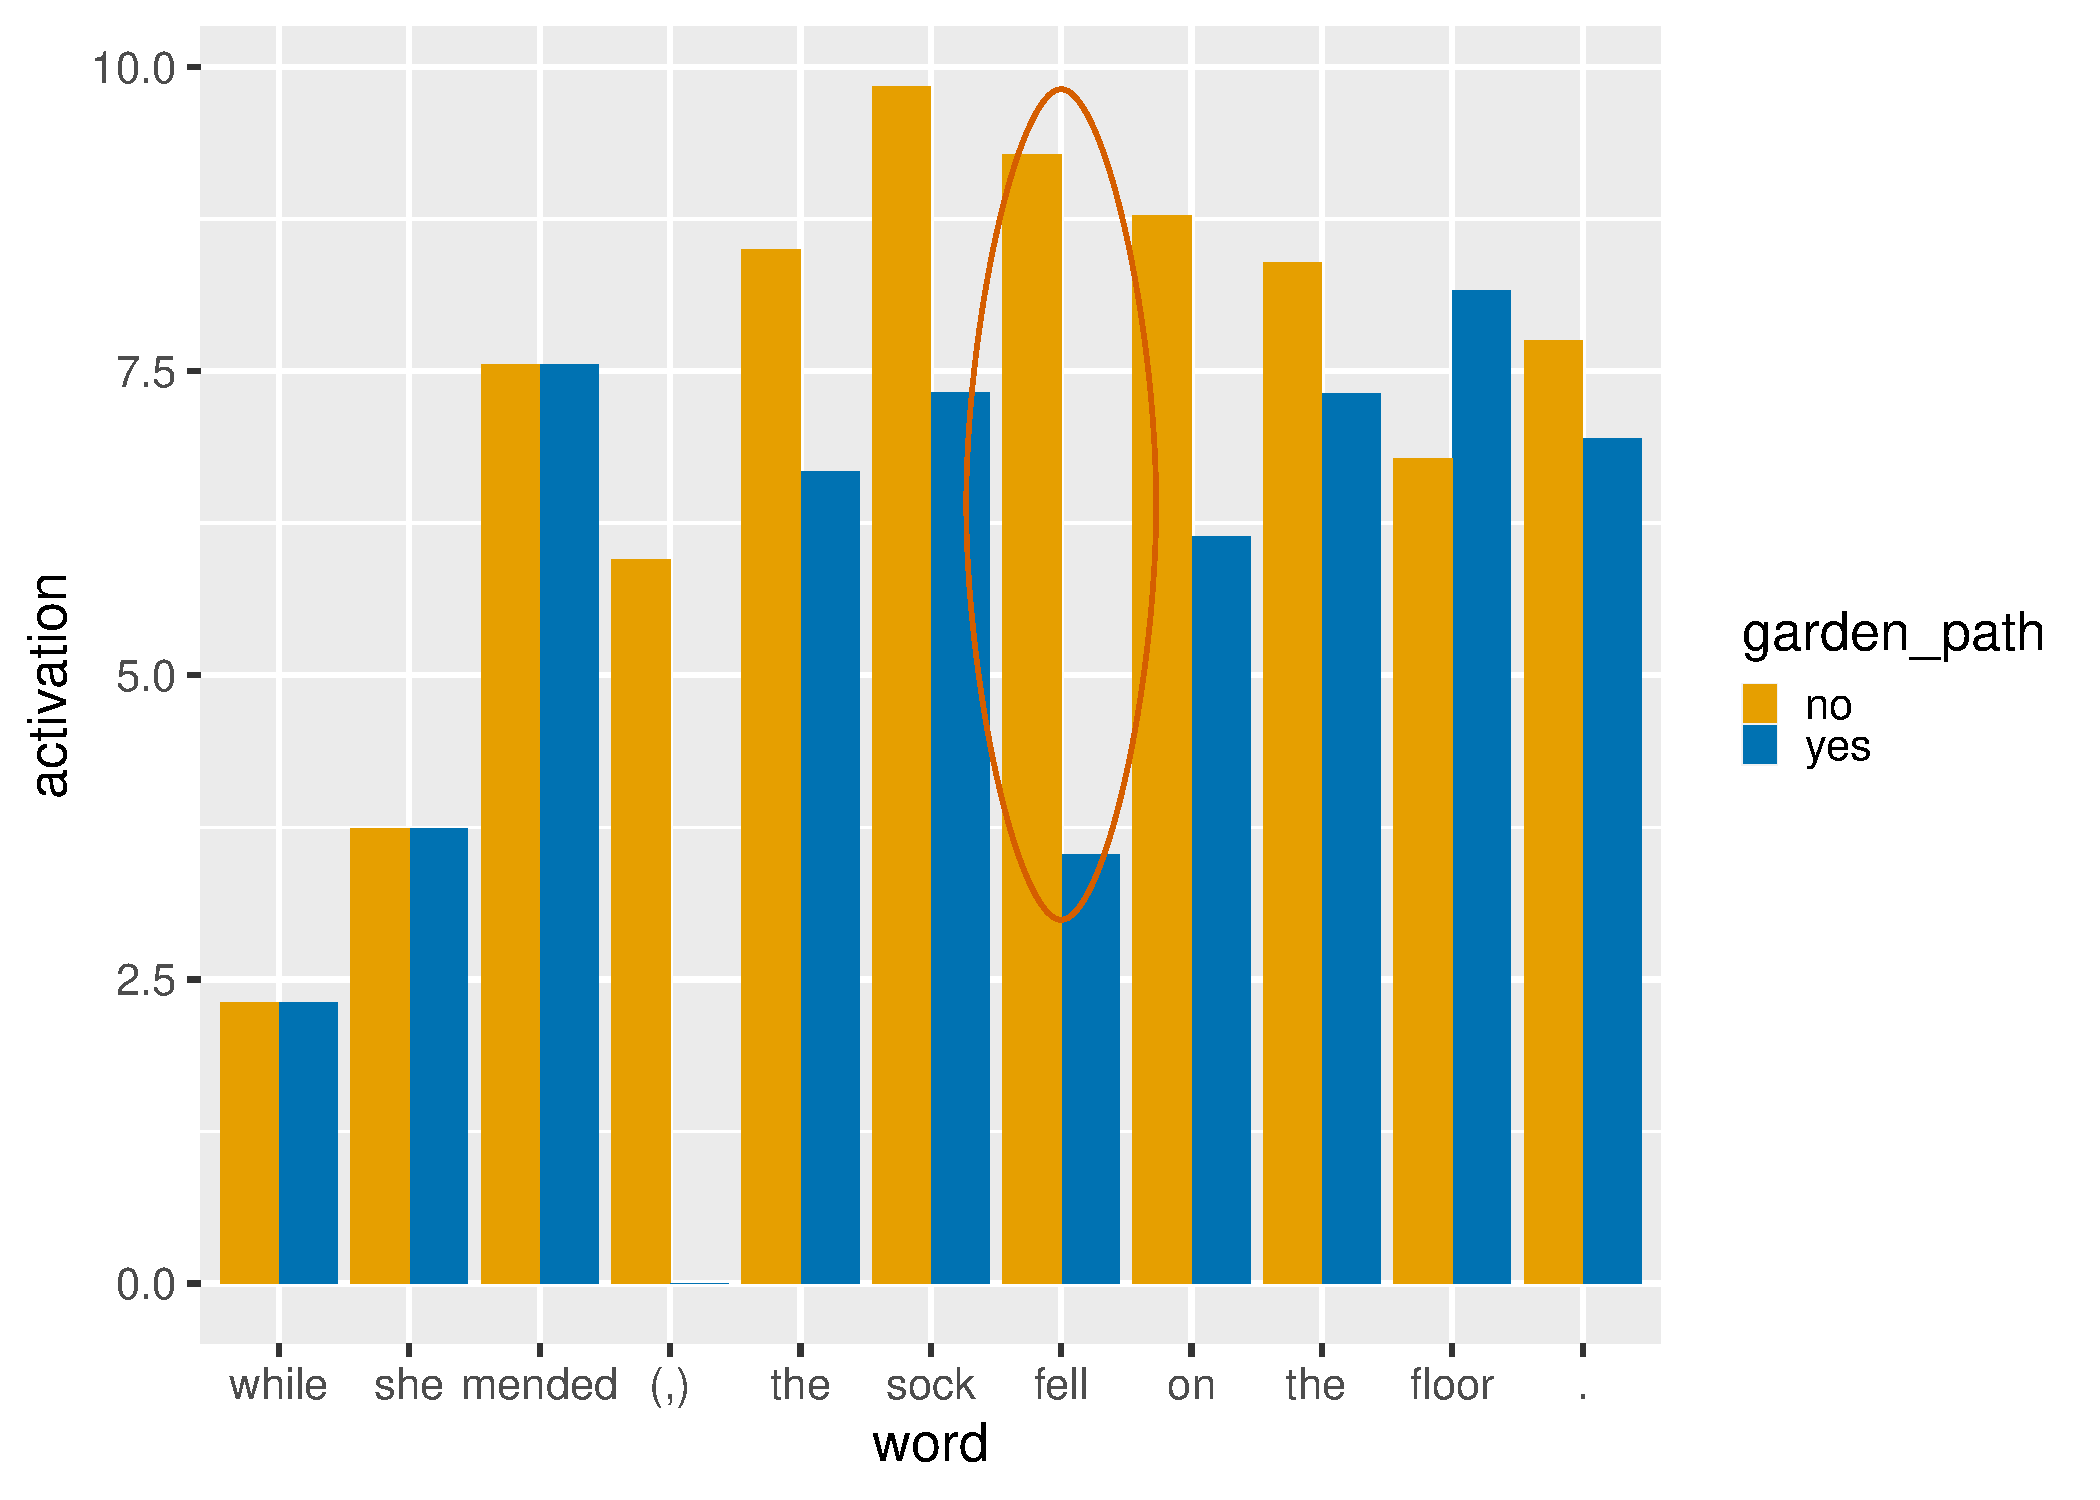
\includegraphics[width=\maxwidth]{figures/unnamed-chunk-6-1} 

\end{knitrout}

\begin{knitrout}
\definecolor{shadecolor}{rgb}{0.969, 0.969, 0.969}\color{fgcolor}\begin{kframe}
\begin{alltt}
\hlstd{case3} \hlkwb{<-} \hlkwd{subset}\hlstd{(gp, sent_nr} \hlopt{==} \hlnum{5} \hlopt{|} \hlstd{sent_nr} \hlopt{==} \hlnum{6}\hlstd{)}

\hlkwd{str}\hlstd{(case3)}
\end{alltt}
\begin{verbatim}
## 'data.frame':	17 obs. of  9 variables:
##  $ activation      : num  3.98 4.98 7.6 7.04 4.82 ...
##  $ position        : int  1 2 3 4 5 6 7 8 1 2 ...
##  $ word            : Factor w/ 36 levels ",",".","a","are",..: 17 12 18 31 10 4 22 2 17 12 ...
##  $ sent_nr         : int  5 5 5 5 5 5 5 5 6 6 ...
##  $ retrieve_wh     : Factor w/ 1 level "None": 1 1 1 1 1 1 1 1 1 1 ...
##  $ reanalysis      : Factor w/ 2 levels "no","yes": 1 1 1 1 1 1 2 1 1 1 ...
##  $ agreeing_actions: num  2 2.5 3 3 20 ...
##  $ matching_fs     : num  11.67 9.58 9.33 9 7 ...
##  $ fan_size        : num  1030551 1244206 1371128 1431177 12391731 ...
\end{verbatim}
\begin{alltt}
\hlstd{case3}\hlopt{$}\hlstd{word} \hlkwb{<-} \hlkwd{as.character}\hlstd{(case3}\hlopt{$}\hlstd{word)}

\hlstd{case3}\hlopt{$}\hlstd{word[}\hlkwd{which}\hlstd{(case3}\hlopt{$}\hlstd{word} \hlopt{==} \hlstr{"that"}\hlstd{)]} \hlkwb{<-} \hlstr{"(that)"}

\hlstd{case3}\hlopt{$}\hlstd{word} \hlkwb{<-} \hlkwd{as.factor}\hlstd{(}\hlkwd{as.character}\hlstd{(case3}\hlopt{$}\hlstd{word))}
\hlkwd{levels}\hlstd{(case3}\hlopt{$}\hlstd{word)}
\end{alltt}
\begin{verbatim}
## [1] "."         "(that)"    "are"       "children"  "convinced"
## [6] "he"        "her"       "noisy"     "tired"
\end{verbatim}
\begin{alltt}
\hlstd{case3}\hlopt{$}\hlstd{garden_path} \hlkwb{<-} \hlstr{"no"}
\hlstd{case3}\hlopt{$}\hlstd{garden_path[}\hlkwd{which}\hlstd{(case3}\hlopt{$}\hlstd{sent} \hlopt{==} \hlnum{5}\hlstd{)]} \hlkwb{<-} \hlstr{"yes"}

\hlstd{case3} \hlkwb{<-} \hlkwd{rbind}\hlstd{(case3,} \hlkwd{data.frame}\hlstd{(}\hlkwc{activation} \hlstd{=} \hlnum{0}\hlstd{,} \hlkwc{position} \hlstd{=} \hlnum{0}\hlstd{,} \hlkwc{word} \hlstd{=} \hlstr{"(that)"}\hlstd{,}
    \hlkwc{sent_nr} \hlstd{=} \hlnum{5}\hlstd{,} \hlkwc{retrieve_wh} \hlstd{=} \hlstr{"None"}\hlstd{,} \hlkwc{reanalysis} \hlstd{=} \hlstr{"no"}\hlstd{,} \hlkwc{agreeing_actions} \hlstd{=} \hlnum{0}\hlstd{,}
    \hlkwc{matching_fs} \hlstd{=} \hlnum{0}\hlstd{,} \hlkwc{fan_size} \hlstd{=} \hlnum{0}\hlstd{,} \hlkwc{garden_path} \hlstd{=} \hlstr{"yes"}\hlstd{))}

\hlstd{case3}\hlopt{$}\hlstd{gp} \hlkwb{<-} \hlnum{NA}
\hlstd{case3}\hlopt{$}\hlstd{gp[}\hlkwd{which}\hlstd{(case3}\hlopt{$}\hlstd{word} \hlopt{==} \hlstr{"are"}\hlstd{)]} \hlkwb{<-} \hlstr{"yes"}

\hlstd{ordered_levels} \hlkwb{<-} \hlkwd{as.numeric}\hlstd{(}\hlkwd{subset}\hlstd{(case3, sent_nr} \hlopt{==} \hlnum{6}\hlstd{)}\hlopt{$}\hlstd{word)}

\hlstd{case3}\hlopt{$}\hlstd{word} \hlkwb{<-} \hlkwd{factor}\hlstd{(case3}\hlopt{$}\hlstd{word,} \hlkwd{levels}\hlstd{(case3}\hlopt{$}\hlstd{word)[ordered_levels])}
\hlkwd{levels}\hlstd{(case3}\hlopt{$}\hlstd{word)}
\end{alltt}
\begin{verbatim}
## [1] "he"        "convinced" "her"       "(that)"    "tired"    
## [6] "children"  "are"       "noisy"     "."
\end{verbatim}
\begin{alltt}
\hlkwd{str}\hlstd{(case3)}
\end{alltt}
\begin{verbatim}
## 'data.frame':	18 obs. of  11 variables:
##  $ activation      : num  3.98 4.98 7.6 7.04 4.82 ...
##  $ position        : num  1 2 3 4 5 6 7 8 1 2 ...
##  $ word            : Factor w/ 9 levels "he","convinced",..: 1 2 3 5 6 7 8 9 1 2 ...
##  $ sent_nr         : num  5 5 5 5 5 5 5 5 6 6 ...
##  $ retrieve_wh     : Factor w/ 1 level "None": 1 1 1 1 1 1 1 1 1 1 ...
##  $ reanalysis      : Factor w/ 2 levels "no","yes": 1 1 1 1 1 1 2 1 1 1 ...
##  $ agreeing_actions: num  2 2.5 3 3 20 ...
##  $ matching_fs     : num  11.67 9.58 9.33 9 7 ...
##  $ fan_size        : num  1030551 1244206 1371128 1431177 12391731 ...
##  $ garden_path     : chr  "yes" "yes" "yes" "yes" ...
##  $ gp              : chr  NA NA NA NA ...
\end{verbatim}
\begin{alltt}
\hlstd{g1} \hlkwb{<-} \hlkwd{ggplot}\hlstd{(case3,} \hlkwd{aes}\hlstd{(}\hlkwc{x} \hlstd{= word,} \hlkwc{y} \hlstd{= activation,} \hlkwc{fill} \hlstd{= garden_path,} \hlkwc{group} \hlstd{= garden_path))}
\hlstd{g1} \hlkwb{<-} \hlstd{g1} \hlopt{+} \hlkwd{geom_bar}\hlstd{(}\hlkwc{stat} \hlstd{=} \hlstr{"identity"}\hlstd{,} \hlkwc{position} \hlstd{=} \hlstr{"dodge"}\hlstd{)}
\hlstd{g1} \hlkwb{<-} \hlstd{g1} \hlopt{+} \hlkwd{geom_encircle}\hlstd{(}\hlkwc{data} \hlstd{=} \hlkwd{subset}\hlstd{(case3, gp} \hlopt{==} \hlstr{"yes"}\hlstd{),} \hlkwd{aes}\hlstd{(word, activation),}
    \hlkwc{inherit.aes} \hlstd{=} \hlnum{FALSE}\hlstd{,} \hlkwc{s_shape} \hlstd{=} \hlnum{0}\hlstd{,} \hlkwc{spread} \hlstd{=} \hlnum{0.03}\hlstd{,} \hlkwc{size} \hlstd{=} \hlnum{3}\hlstd{,} \hlkwc{color} \hlstd{=} \hlstr{"#D55E00"}\hlstd{)}
\hlstd{g1} \hlkwb{<-} \hlstd{g1} \hlopt{+} \hlkwd{theme_gray}\hlstd{(}\hlnum{26}\hlstd{)} \hlopt{+} \hlkwd{scale_fill_manual}\hlstd{(}\hlkwc{values} \hlstd{= cbPalette)}
\end{alltt}
\end{kframe}
\end{knitrout}

\begin{knitrout}
\definecolor{shadecolor}{rgb}{0.969, 0.969, 0.969}\color{fgcolor}
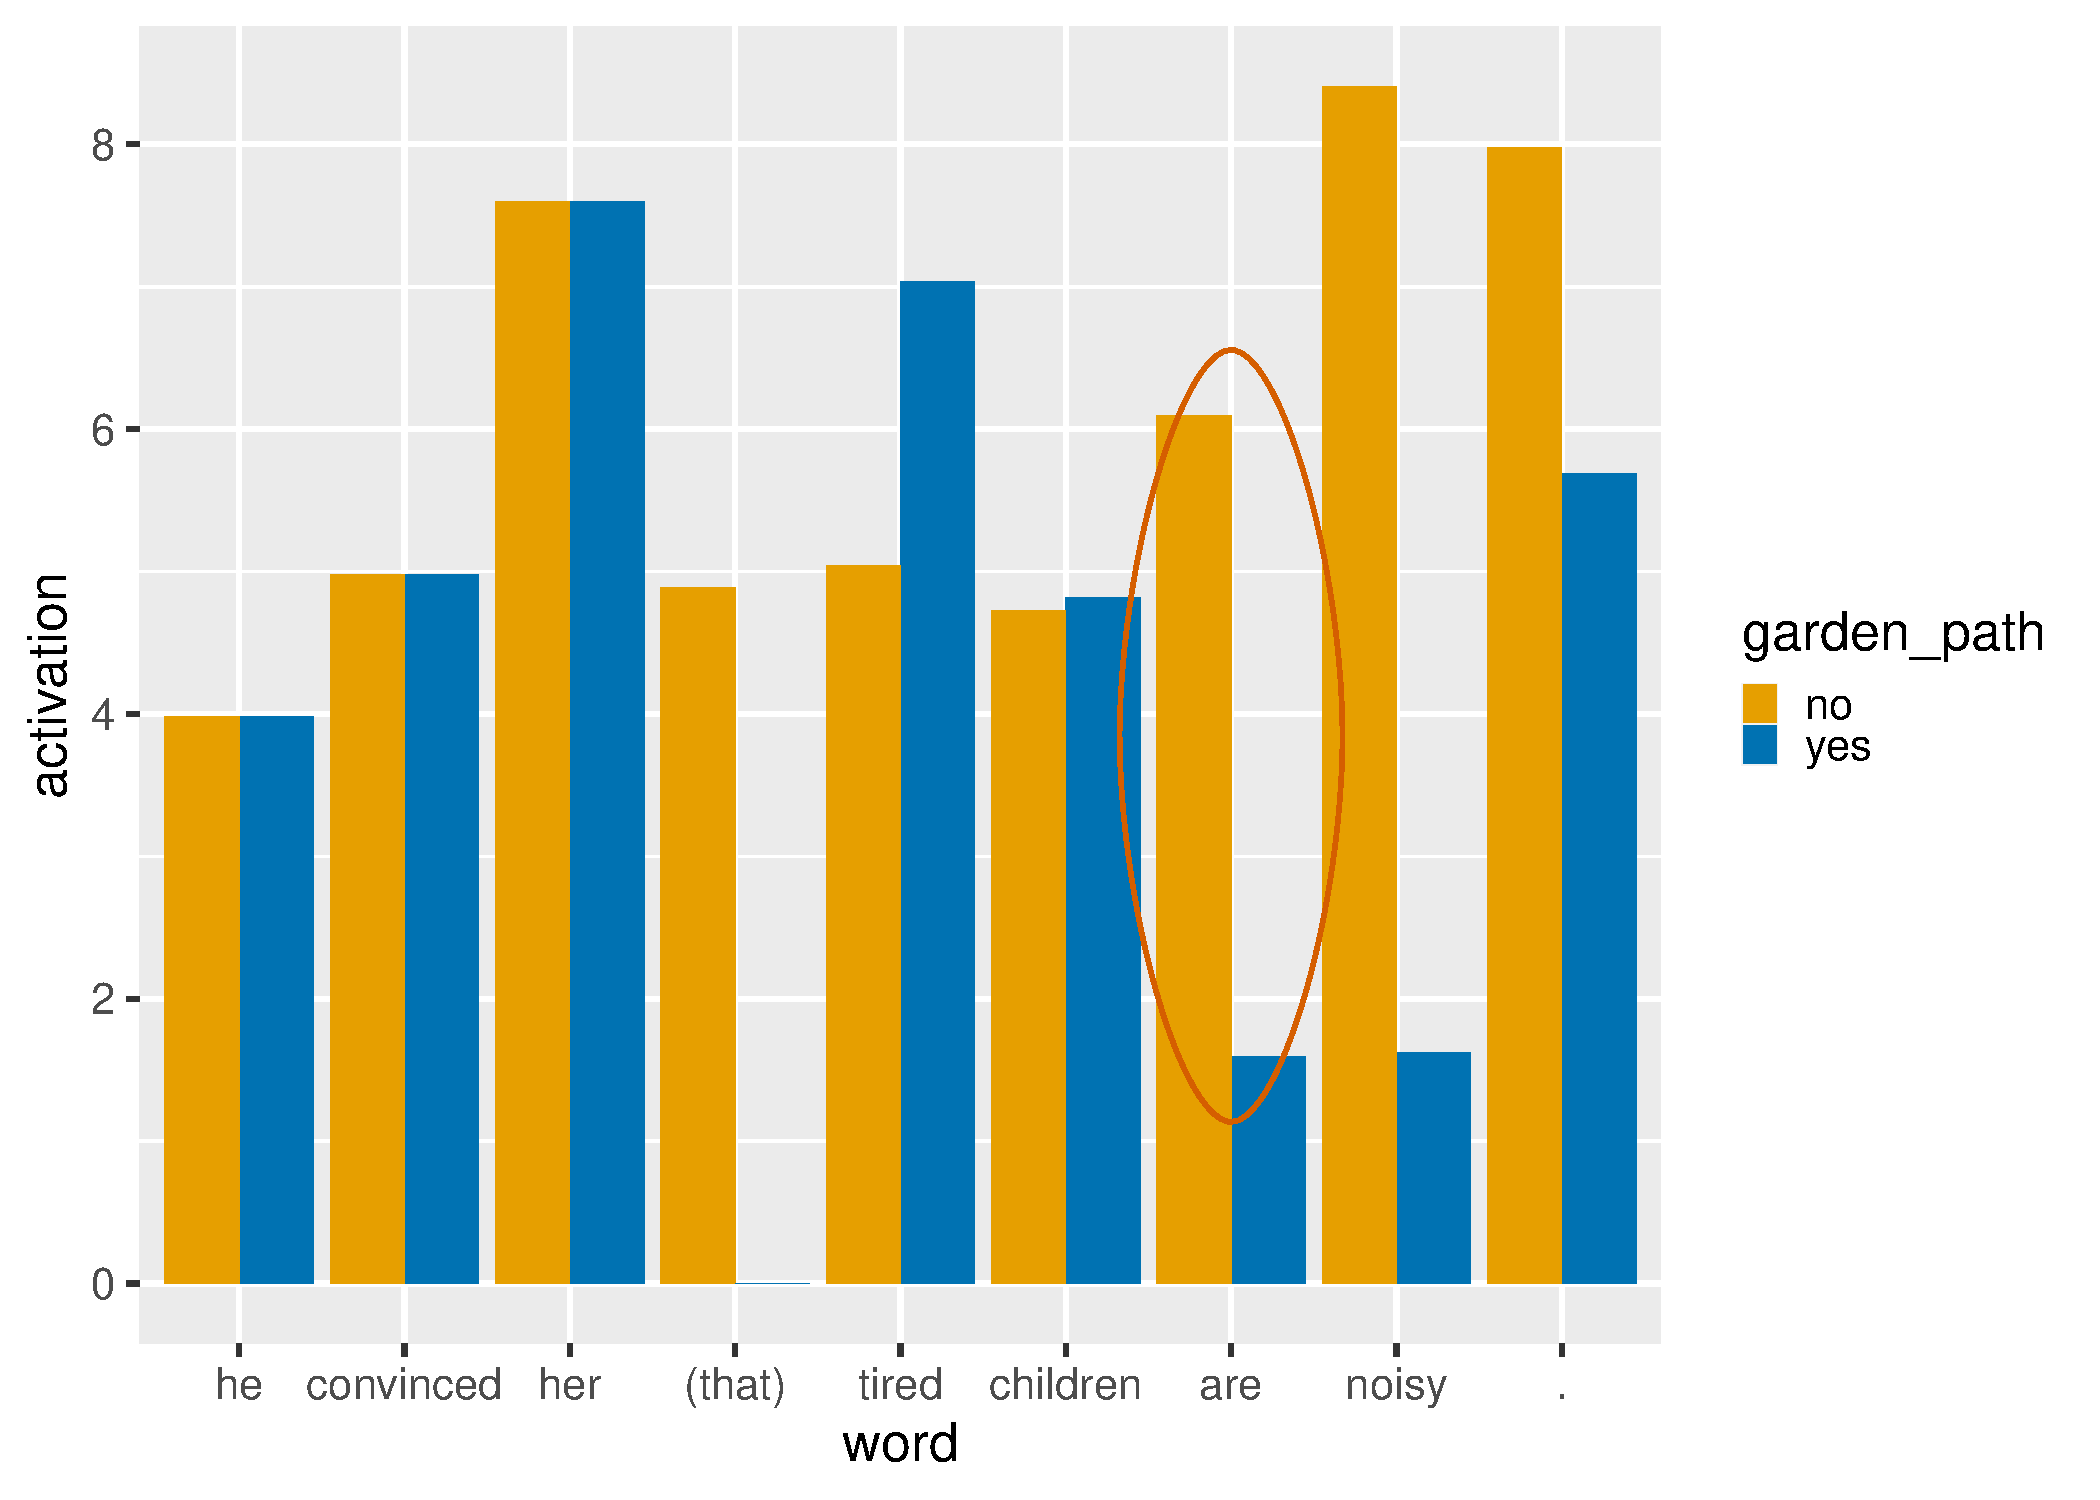
\includegraphics[width=\maxwidth]{figures/unnamed-chunk-8-1} 

\end{knitrout}

\begin{knitrout}
\definecolor{shadecolor}{rgb}{0.969, 0.969, 0.969}\color{fgcolor}\begin{kframe}
\begin{alltt}
\hlstd{case4} \hlkwb{<-} \hlkwd{subset}\hlstd{(gp, sent_nr} \hlopt{==} \hlnum{7} \hlopt{|} \hlstd{sent_nr} \hlopt{==} \hlnum{8}\hlstd{)}

\hlkwd{str}\hlstd{(case4)}
\end{alltt}
\begin{verbatim}
## 'data.frame':	21 obs. of  9 variables:
##  $ activation      : num  4.05 5.06 6.14 8.64 7.43 ...
##  $ position        : int  1 2 3 4 5 6 7 8 9 10 ...
##  $ word            : Factor w/ 36 levels ",",".","a","are",..: 27 16 30 9 30 13 8 3 5 2 ...
##  $ sent_nr         : int  7 7 7 7 7 7 7 7 7 7 ...
##  $ retrieve_wh     : Factor w/ 1 level "None": 1 1 1 1 1 1 1 1 1 1 ...
##  $ reanalysis      : Factor w/ 2 levels "no","yes": 1 1 1 2 1 1 1 1 2 1 ...
##  $ agreeing_actions: num  2 2.5 2 3 3 ...
##  $ matching_fs     : num  11.17 9.33 16 10.33 8.78 ...
##  $ fan_size        : num  1048230 1252370 822317 1296018 1537815 ...
\end{verbatim}
\begin{alltt}
\hlstd{case4}\hlopt{$}\hlstd{word} \hlkwb{<-} \hlkwd{as.character}\hlstd{(case4}\hlopt{$}\hlstd{word)}

\hlstd{case4}\hlopt{$}\hlstd{word[}\hlkwd{which}\hlstd{(case4}\hlopt{$}\hlstd{position} \hlopt{==} \hlnum{5} \hlopt{&} \hlstd{case4}\hlopt{$}\hlstd{sent_nr} \hlopt{==} \hlnum{7}\hlstd{)]} \hlkwb{<-} \hlstr{"the "}
\hlstd{case4}\hlopt{$}\hlstd{word[}\hlkwd{which}\hlstd{(case4}\hlopt{$}\hlstd{position} \hlopt{==} \hlnum{6} \hlopt{&} \hlstd{case4}\hlopt{$}\hlstd{sent_nr} \hlopt{==} \hlnum{8}\hlstd{)]} \hlkwb{<-} \hlstr{"the "}
\hlstd{case4}\hlopt{$}\hlstd{word[}\hlkwd{which}\hlstd{(case4}\hlopt{$}\hlstd{word} \hlopt{==} \hlstr{"that"}\hlstd{)]} \hlkwb{<-} \hlstr{"(that)"}

\hlstd{case4}\hlopt{$}\hlstd{word} \hlkwb{<-} \hlkwd{as.factor}\hlstd{(}\hlkwd{as.character}\hlstd{(case4}\hlopt{$}\hlstd{word))}
\hlkwd{levels}\hlstd{(case4}\hlopt{$}\hlstd{word)}
\end{alltt}
\begin{verbatim}
##  [1] "."       "(that)"  "a"       "bandage" "bit"     "boy"     "dog"    
##  [8] "gave"    "she"     "the"     "the "
\end{verbatim}
\begin{alltt}
\hlstd{case4}\hlopt{$}\hlstd{garden_path} \hlkwb{<-} \hlstr{"no"}
\hlstd{case4}\hlopt{$}\hlstd{garden_path[}\hlkwd{which}\hlstd{(case4}\hlopt{$}\hlstd{sent} \hlopt{==} \hlnum{7}\hlstd{)]} \hlkwb{<-} \hlstr{"yes"}

\hlstd{case4} \hlkwb{<-} \hlkwd{rbind}\hlstd{(case4,} \hlkwd{data.frame}\hlstd{(}\hlkwc{activation} \hlstd{=} \hlnum{0}\hlstd{,} \hlkwc{position} \hlstd{=} \hlnum{0}\hlstd{,} \hlkwc{word} \hlstd{=} \hlstr{"(that)"}\hlstd{,}
    \hlkwc{sent_nr} \hlstd{=} \hlnum{7}\hlstd{,} \hlkwc{retrieve_wh} \hlstd{=} \hlstr{"None"}\hlstd{,} \hlkwc{reanalysis} \hlstd{=} \hlstr{"no"}\hlstd{,} \hlkwc{agreeing_actions} \hlstd{=} \hlnum{0}\hlstd{,}
    \hlkwc{matching_fs} \hlstd{=} \hlnum{0}\hlstd{,} \hlkwc{fan_size} \hlstd{=} \hlnum{0}\hlstd{,} \hlkwc{garden_path} \hlstd{=} \hlstr{"yes"}\hlstd{))}

\hlstd{case4}\hlopt{$}\hlstd{gp} \hlkwb{<-} \hlnum{NA}
\hlstd{case4}\hlopt{$}\hlstd{gp[}\hlkwd{which}\hlstd{(case4}\hlopt{$}\hlstd{word} \hlopt{==} \hlstr{"bit"}\hlstd{)]} \hlkwb{<-} \hlstr{"yes"}

\hlstd{ordered_levels} \hlkwb{<-} \hlkwd{as.numeric}\hlstd{(}\hlkwd{subset}\hlstd{(case4, sent_nr} \hlopt{==} \hlnum{8}\hlstd{)}\hlopt{$}\hlstd{word)}

\hlstd{case4}\hlopt{$}\hlstd{word} \hlkwb{<-} \hlkwd{factor}\hlstd{(case4}\hlopt{$}\hlstd{word,} \hlkwd{levels}\hlstd{(case4}\hlopt{$}\hlstd{word)[ordered_levels])}
\hlkwd{levels}\hlstd{(case4}\hlopt{$}\hlstd{word)}
\end{alltt}
\begin{verbatim}
##  [1] "she"     "gave"    "the"     "boy"     "(that)"  "the "    "dog"    
##  [8] "bit"     "a"       "bandage" "."
\end{verbatim}
\begin{alltt}
\hlkwd{str}\hlstd{(case4)}
\end{alltt}
\begin{verbatim}
## 'data.frame':	22 obs. of  11 variables:
##  $ activation      : num  4.05 5.06 6.14 8.64 7.43 ...
##  $ position        : num  1 2 3 4 5 6 7 8 9 10 ...
##  $ word            : Factor w/ 11 levels "she","gave","the",..: 1 2 3 4 6 7 8 9 10 11 ...
##  $ sent_nr         : num  7 7 7 7 7 7 7 7 7 7 ...
##  $ retrieve_wh     : Factor w/ 1 level "None": 1 1 1 1 1 1 1 1 1 1 ...
##  $ reanalysis      : Factor w/ 2 levels "no","yes": 1 1 1 2 1 1 1 1 2 1 ...
##  $ agreeing_actions: num  2 2.5 2 3 3 ...
##  $ matching_fs     : num  11.17 9.33 16 10.33 8.78 ...
##  $ fan_size        : num  1048230 1252370 822317 1296018 1537815 ...
##  $ garden_path     : chr  "yes" "yes" "yes" "yes" ...
##  $ gp              : chr  NA NA NA NA ...
\end{verbatim}
\begin{alltt}
\hlstd{g1} \hlkwb{<-} \hlkwd{ggplot}\hlstd{(case4,} \hlkwd{aes}\hlstd{(}\hlkwc{x} \hlstd{= word,} \hlkwc{y} \hlstd{= activation,} \hlkwc{fill} \hlstd{= garden_path,} \hlkwc{group} \hlstd{= garden_path))}
\hlstd{g1} \hlkwb{<-} \hlstd{g1} \hlopt{+} \hlkwd{geom_bar}\hlstd{(}\hlkwc{stat} \hlstd{=} \hlstr{"identity"}\hlstd{,} \hlkwc{position} \hlstd{=} \hlstr{"dodge"}\hlstd{)}
\hlstd{g1} \hlkwb{<-} \hlstd{g1} \hlopt{+} \hlkwd{geom_encircle}\hlstd{(}\hlkwc{data} \hlstd{=} \hlkwd{subset}\hlstd{(case4, gp} \hlopt{==} \hlstr{"yes"}\hlstd{),} \hlkwd{aes}\hlstd{(word, activation),}
    \hlkwc{inherit.aes} \hlstd{=} \hlnum{FALSE}\hlstd{,} \hlkwc{s_shape} \hlstd{=} \hlnum{0}\hlstd{,} \hlkwc{spread} \hlstd{=} \hlnum{0.03}\hlstd{,} \hlkwc{size} \hlstd{=} \hlnum{3}\hlstd{,} \hlkwc{color} \hlstd{=} \hlstr{"#D55E00"}\hlstd{)}
\hlstd{g1} \hlkwb{<-} \hlstd{g1} \hlopt{+} \hlkwd{theme_gray}\hlstd{(}\hlnum{26}\hlstd{)} \hlopt{+} \hlkwd{scale_fill_manual}\hlstd{(}\hlkwc{values} \hlstd{= cbPalette)}
\end{alltt}
\end{kframe}
\end{knitrout}

\begin{knitrout}
\definecolor{shadecolor}{rgb}{0.969, 0.969, 0.969}\color{fgcolor}
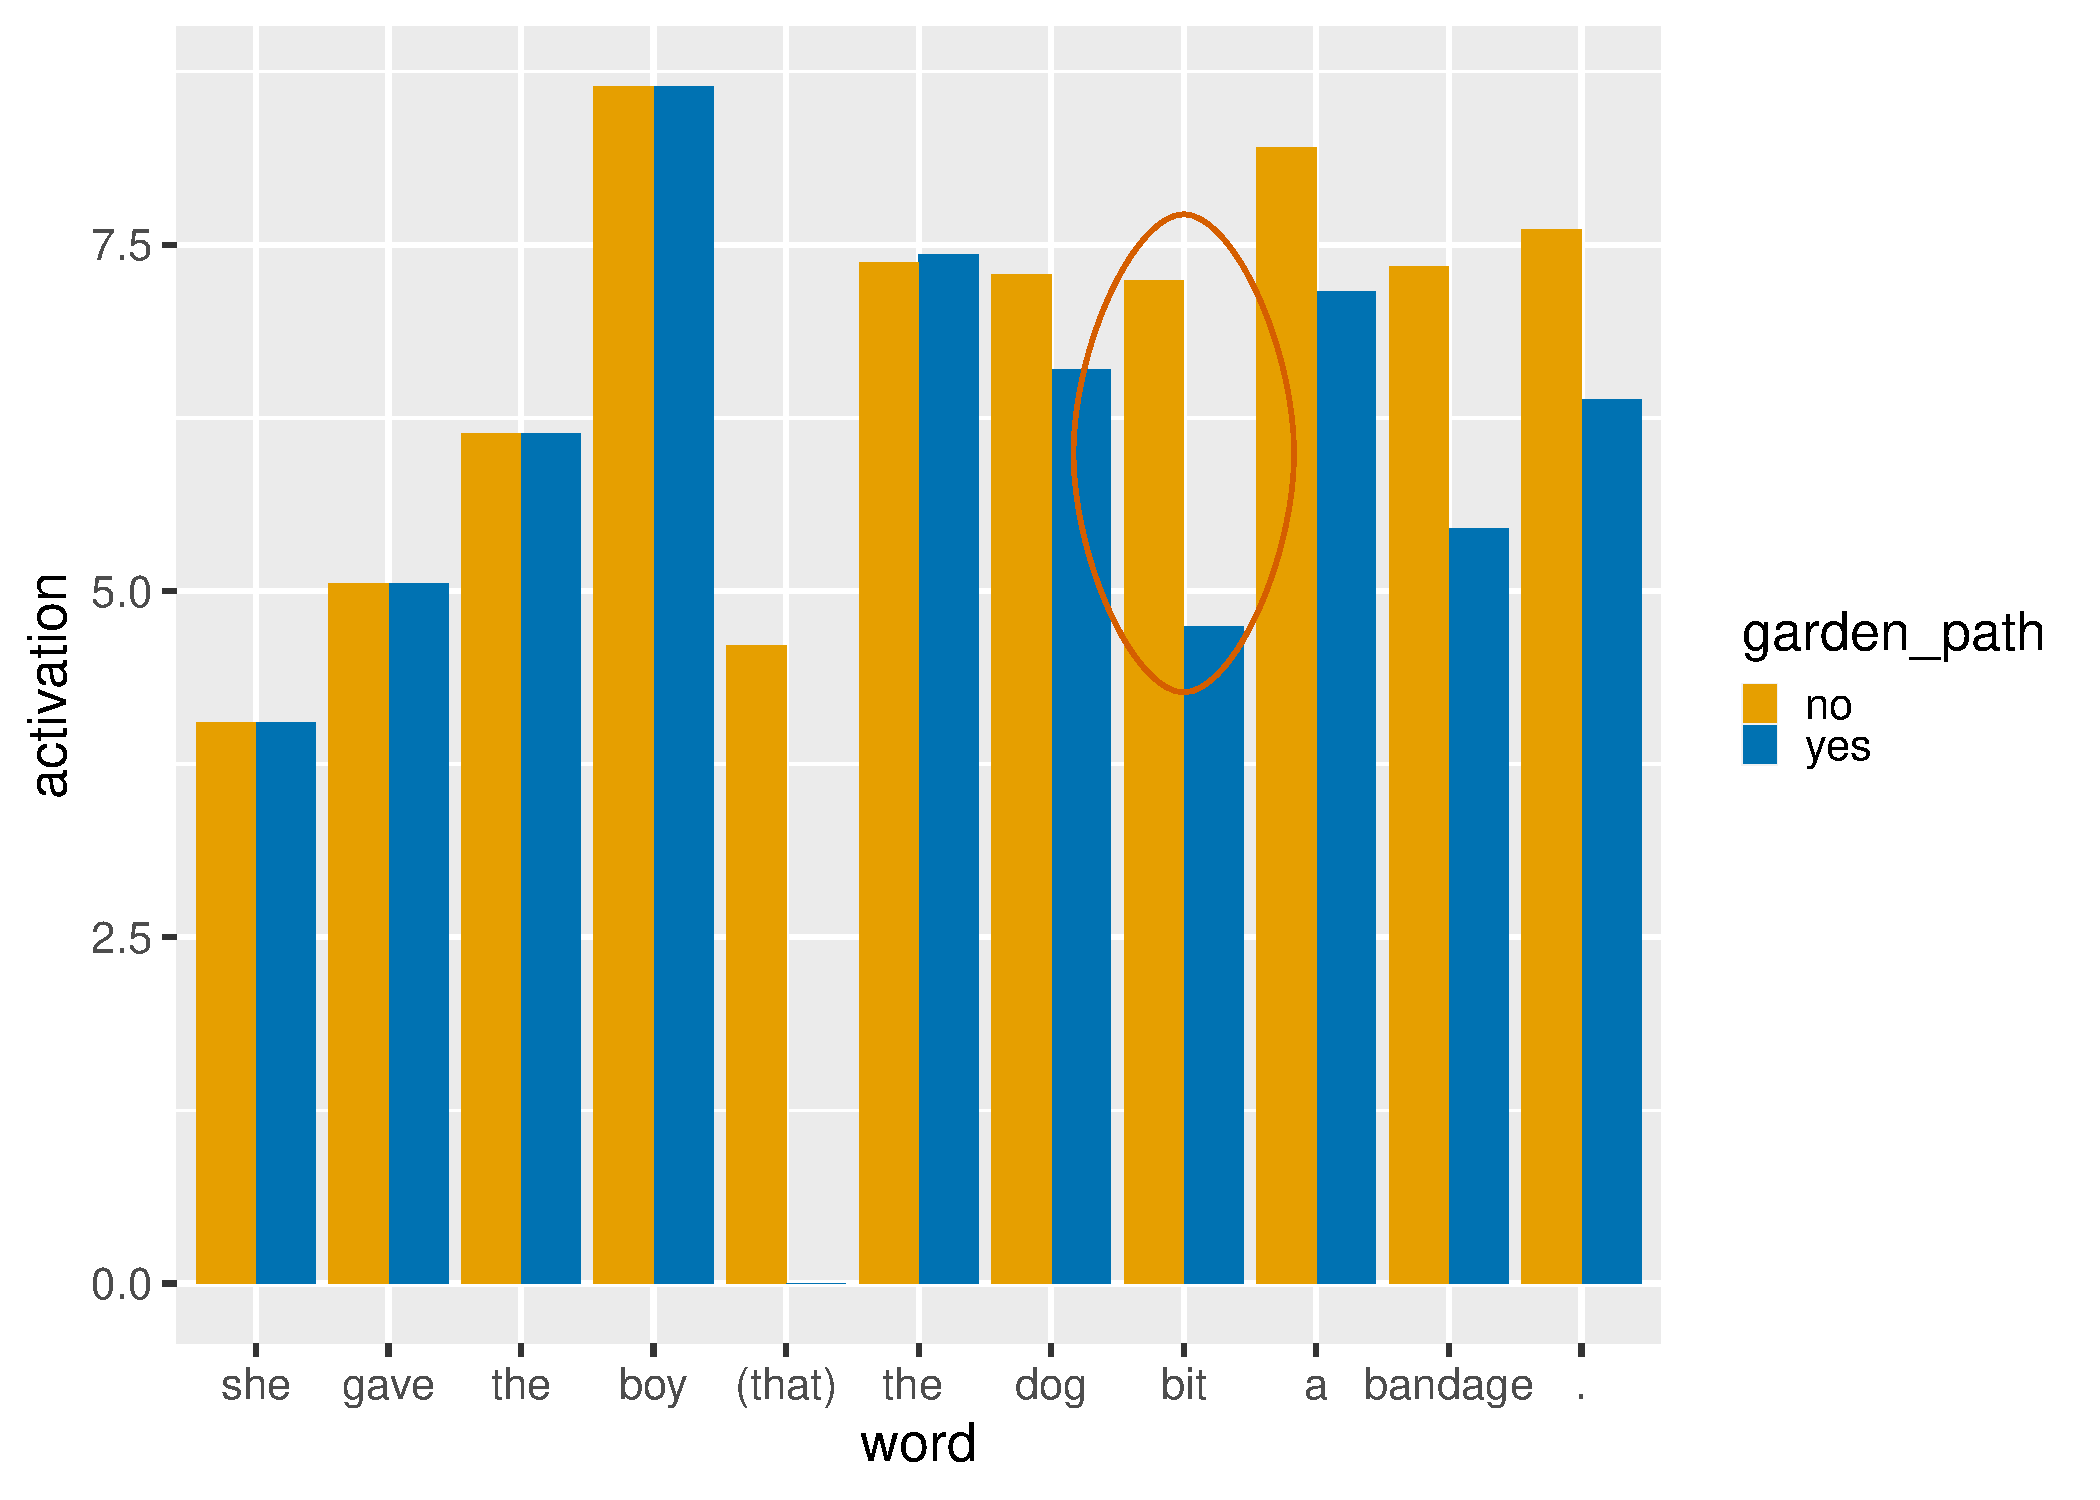
\includegraphics[width=\maxwidth]{figures/unnamed-chunk-10-1} 

\end{knitrout}

\begin{knitrout}
\definecolor{shadecolor}{rgb}{0.969, 0.969, 0.969}\color{fgcolor}\begin{kframe}
\begin{alltt}
\hlstd{case5} \hlkwb{<-} \hlkwd{subset}\hlstd{(gp, sent_nr} \hlopt{==} \hlnum{9} \hlopt{|} \hlstd{sent_nr} \hlopt{==} \hlnum{10}\hlstd{)}

\hlkwd{str}\hlstd{(case5)}
\end{alltt}
\begin{verbatim}
## 'data.frame':	17 obs. of  9 variables:
##  $ activation      : num  2.29 2.4 5.19 5.19 4.62 ...
##  $ position        : int  1 2 3 4 5 6 7 8 1 2 ...
##  $ word            : Factor w/ 36 levels ",",".","a","are",..: 36 18 26 11 35 7 20 2 36 18 ...
##  $ sent_nr         : int  9 9 9 9 9 9 9 9 10 10 ...
##  $ retrieve_wh     : Factor w/ 1 level "None": 1 1 1 1 1 1 1 1 1 1 ...
##  $ reanalysis      : Factor w/ 2 levels "no","yes": 1 1 1 2 1 1 2 1 1 2 ...
##  $ agreeing_actions: num  2 2 3 3 2.33 ...
##  $ matching_fs     : num  7 7.25 7 7 10.17 ...
##  $ fan_size        : num  1322633 1285783 1814393 1817171 1287026 ...
\end{verbatim}
\begin{alltt}
\hlstd{case5}\hlopt{$}\hlstd{word} \hlkwb{<-} \hlkwd{as.character}\hlstd{(case5}\hlopt{$}\hlstd{word)}

\hlstd{case5}\hlopt{$}\hlstd{word[}\hlkwd{which}\hlstd{(case5}\hlopt{$}\hlstd{word} \hlopt{==} \hlstr{","}\hlstd{)]} \hlkwb{<-} \hlstr{"(,)"}
\hlstd{case5}\hlopt{$}\hlstd{word} \hlkwb{<-} \hlkwd{as.factor}\hlstd{(}\hlkwd{as.character}\hlstd{(case5}\hlopt{$}\hlstd{word))}
\hlkwd{levels}\hlstd{(case5}\hlopt{$}\hlstd{word)}
\end{alltt}
\begin{verbatim}
## [1] "."             "(,)"           "be"            "contributions"
## [5] "her"           "inadequate"    "rich"          "will"         
## [9] "without"
\end{verbatim}
\begin{alltt}
\hlstd{case5}\hlopt{$}\hlstd{garden_path} \hlkwb{<-} \hlstr{"no"}
\hlstd{case5}\hlopt{$}\hlstd{garden_path[}\hlkwd{which}\hlstd{(case5}\hlopt{$}\hlstd{sent} \hlopt{==} \hlnum{9}\hlstd{)]} \hlkwb{<-} \hlstr{"yes"}

\hlstd{case5} \hlkwb{<-} \hlkwd{rbind}\hlstd{(case5,} \hlkwd{data.frame}\hlstd{(}\hlkwc{activation} \hlstd{=} \hlnum{0}\hlstd{,} \hlkwc{position} \hlstd{=} \hlnum{0}\hlstd{,} \hlkwc{word} \hlstd{=} \hlstr{"(,)"}\hlstd{,}
    \hlkwc{sent_nr} \hlstd{=} \hlnum{9}\hlstd{,} \hlkwc{retrieve_wh} \hlstd{=} \hlstr{"None"}\hlstd{,} \hlkwc{reanalysis} \hlstd{=} \hlstr{"no"}\hlstd{,} \hlkwc{agreeing_actions} \hlstd{=} \hlnum{0}\hlstd{,}
    \hlkwc{matching_fs} \hlstd{=} \hlnum{0}\hlstd{,} \hlkwc{fan_size} \hlstd{=} \hlnum{0}\hlstd{,} \hlkwc{garden_path} \hlstd{=} \hlstr{"yes"}\hlstd{))}

\hlstd{case5}\hlopt{$}\hlstd{gp} \hlkwb{<-} \hlnum{NA}
\hlstd{case5}\hlopt{$}\hlstd{gp[}\hlkwd{which}\hlstd{(case5}\hlopt{$}\hlstd{word} \hlopt{==} \hlstr{"will"}\hlstd{)]} \hlkwb{<-} \hlstr{"yes"}

\hlstd{ordered_levels} \hlkwb{<-} \hlkwd{as.numeric}\hlstd{(}\hlkwd{subset}\hlstd{(case5, sent_nr} \hlopt{==} \hlnum{10}\hlstd{)}\hlopt{$}\hlstd{word)}

\hlstd{case5}\hlopt{$}\hlstd{word} \hlkwb{<-} \hlkwd{factor}\hlstd{(case5}\hlopt{$}\hlstd{word,} \hlkwd{levels}\hlstd{(case5}\hlopt{$}\hlstd{word)[ordered_levels])}
\hlkwd{levels}\hlstd{(case5}\hlopt{$}\hlstd{word)}
\end{alltt}
\begin{verbatim}
## [1] "without"       "her"           "(,)"           "rich"         
## [5] "contributions" "will"          "be"            "inadequate"   
## [9] "."
\end{verbatim}
\begin{alltt}
\hlkwd{str}\hlstd{(case5)}
\end{alltt}
\begin{verbatim}
## 'data.frame':	18 obs. of  11 variables:
##  $ activation      : num  2.29 2.4 5.19 5.19 4.62 ...
##  $ position        : num  1 2 3 4 5 6 7 8 1 2 ...
##  $ word            : Factor w/ 9 levels "without","her",..: 1 2 4 5 6 7 8 9 1 2 ...
##  $ sent_nr         : num  9 9 9 9 9 9 9 9 10 10 ...
##  $ retrieve_wh     : Factor w/ 1 level "None": 1 1 1 1 1 1 1 1 1 1 ...
##  $ reanalysis      : Factor w/ 2 levels "no","yes": 1 1 1 2 1 1 2 1 1 2 ...
##  $ agreeing_actions: num  2 2 3 3 2.33 ...
##  $ matching_fs     : num  7 7.25 7 7 10.17 ...
##  $ fan_size        : num  1322633 1285783 1814393 1817171 1287026 ...
##  $ garden_path     : chr  "yes" "yes" "yes" "yes" ...
##  $ gp              : chr  NA NA NA NA ...
\end{verbatim}
\begin{alltt}
\hlstd{g1} \hlkwb{<-} \hlkwd{ggplot}\hlstd{(case5,} \hlkwd{aes}\hlstd{(}\hlkwc{x} \hlstd{= word,} \hlkwc{y} \hlstd{= activation,} \hlkwc{fill} \hlstd{= garden_path,} \hlkwc{group} \hlstd{= garden_path))}
\hlstd{g1} \hlkwb{<-} \hlstd{g1} \hlopt{+} \hlkwd{geom_bar}\hlstd{(}\hlkwc{stat} \hlstd{=} \hlstr{"identity"}\hlstd{,} \hlkwc{position} \hlstd{=} \hlstr{"dodge"}\hlstd{)}
\hlstd{g1} \hlkwb{<-} \hlstd{g1} \hlopt{+} \hlkwd{geom_encircle}\hlstd{(}\hlkwc{data} \hlstd{=} \hlkwd{subset}\hlstd{(case5, gp} \hlopt{==} \hlstr{"yes"}\hlstd{),} \hlkwd{aes}\hlstd{(word, activation),}
    \hlkwc{inherit.aes} \hlstd{=} \hlnum{FALSE}\hlstd{,} \hlkwc{s_shape} \hlstd{=} \hlnum{0}\hlstd{,} \hlkwc{spread} \hlstd{=} \hlnum{0.03}\hlstd{,} \hlkwc{size} \hlstd{=} \hlnum{3}\hlstd{,} \hlkwc{color} \hlstd{=} \hlstr{"#D55E00"}\hlstd{)}
\hlstd{g1} \hlkwb{<-} \hlstd{g1} \hlopt{+} \hlkwd{theme_gray}\hlstd{(}\hlnum{26}\hlstd{)} \hlopt{+} \hlkwd{scale_fill_manual}\hlstd{(}\hlkwc{values} \hlstd{= cbPalette)}
\end{alltt}
\end{kframe}
\end{knitrout}

\begin{knitrout}
\definecolor{shadecolor}{rgb}{0.969, 0.969, 0.969}\color{fgcolor}
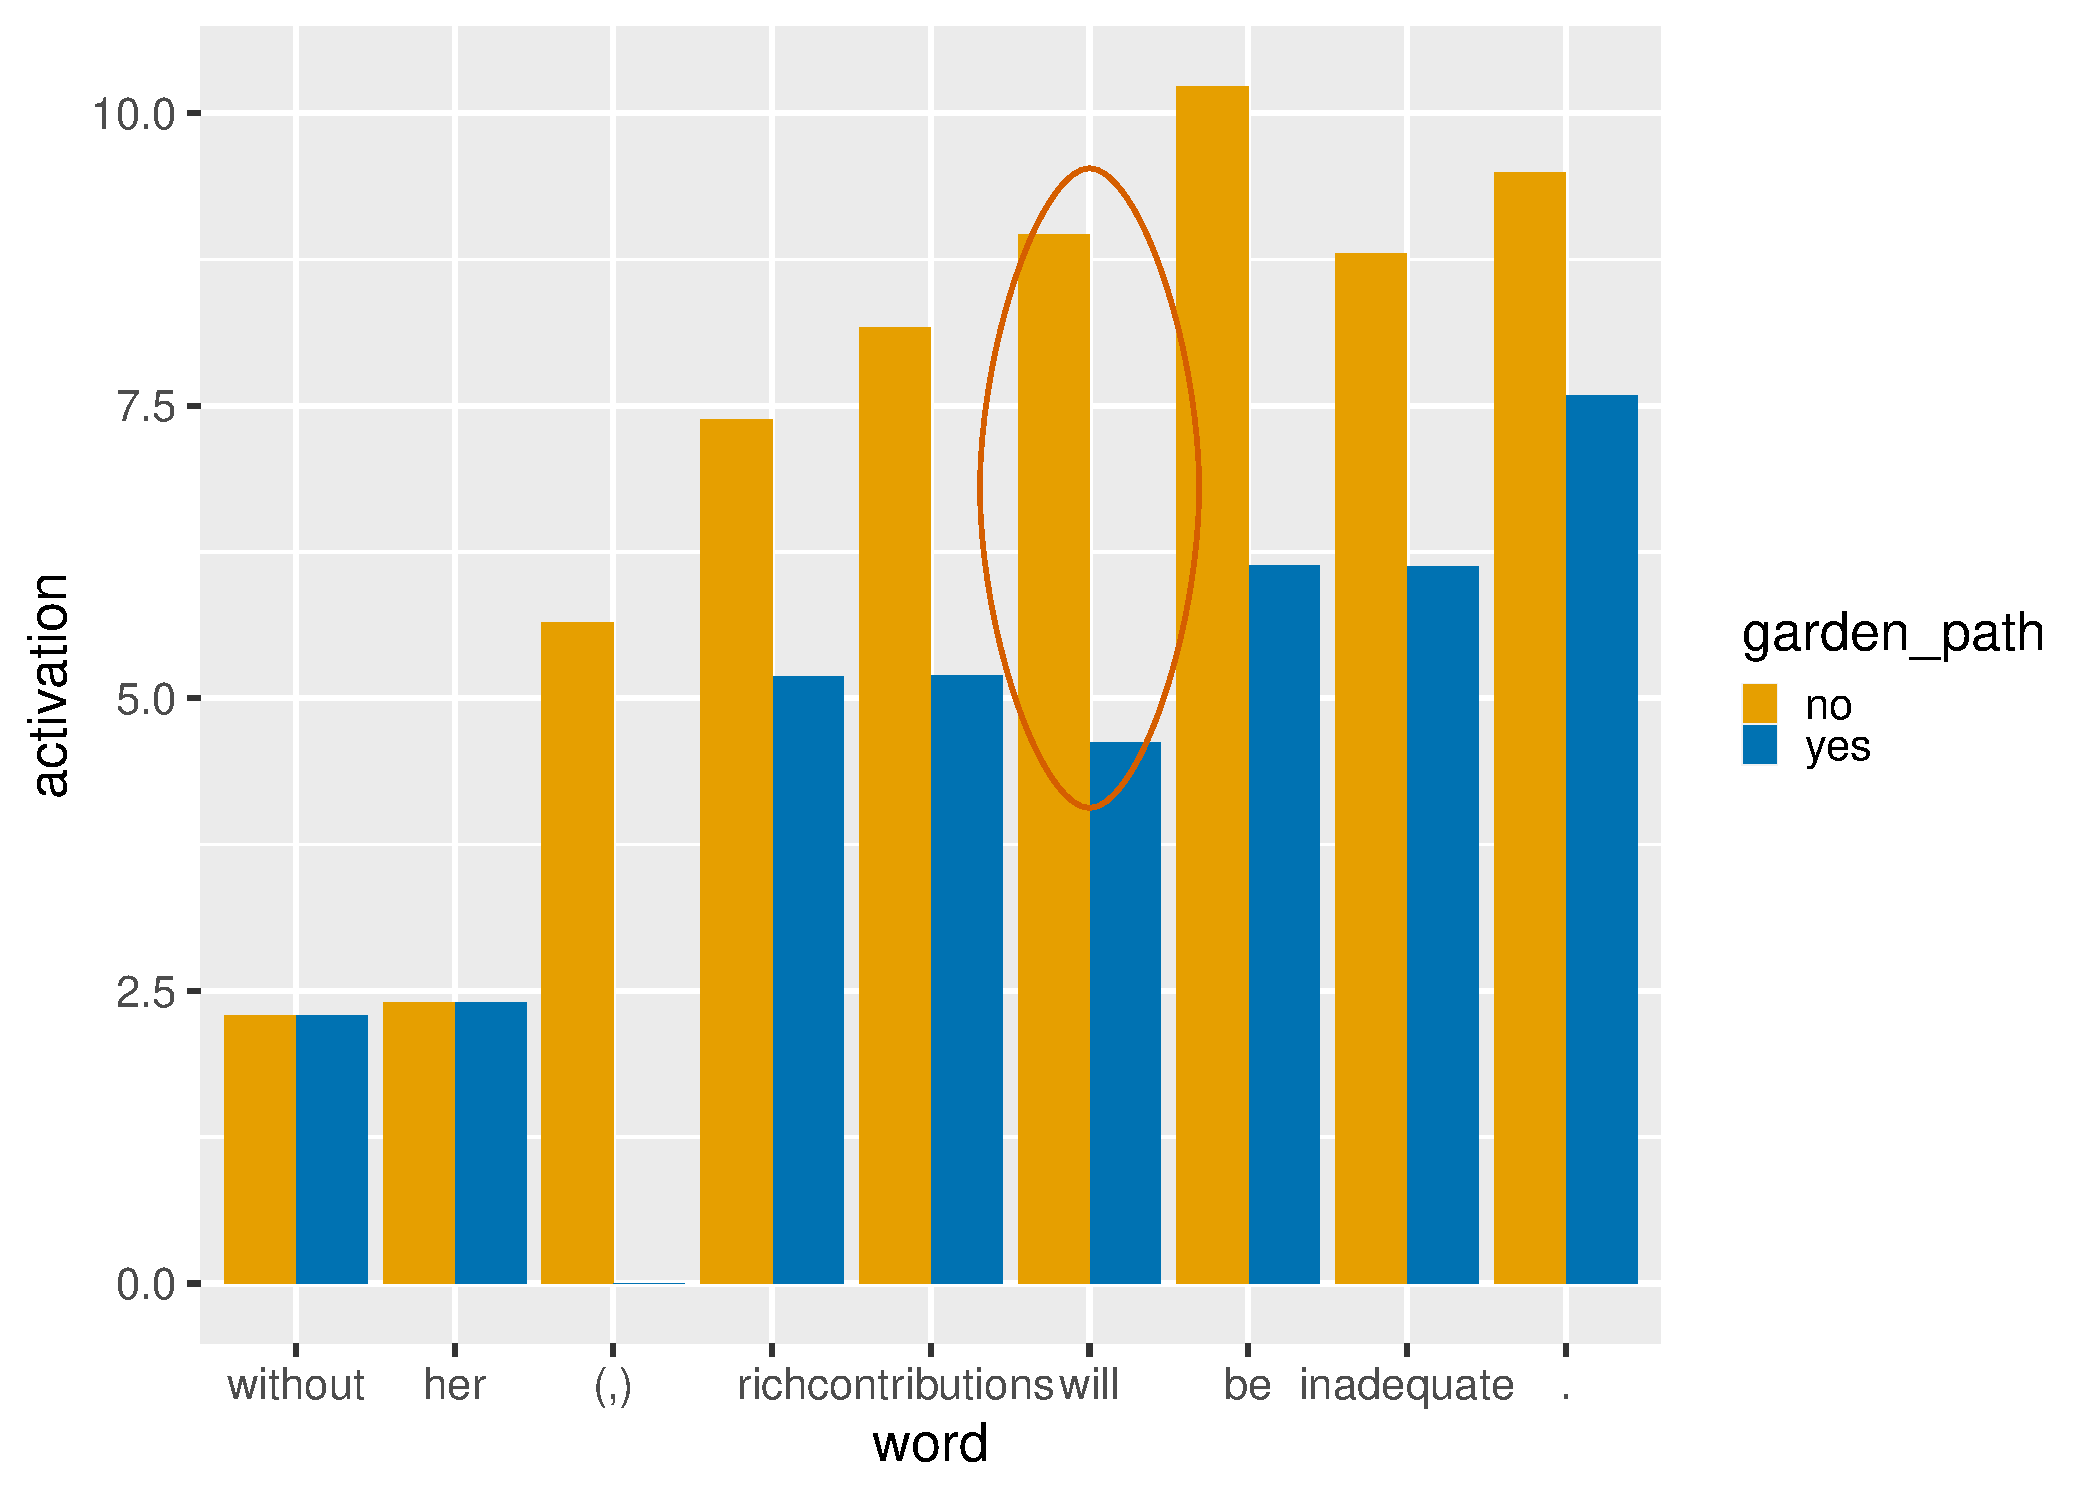
\includegraphics[width=\maxwidth]{figures/unnamed-chunk-12-1} 

\end{knitrout}

\end{document}
